% BrickForge paper. Build: `make paper` (figures via paper/scripts/figs.py, PDF via tectonic).
\documentclass[10pt]{article}
\usepackage[margin=0.95in]{geometry}
\usepackage{newtxtext,newtxmath}  % newtxmath supplies the AMS symbols; amssymb would clash on \Bbbk
\usepackage{amsmath}
\usepackage{booktabs}
\usepackage{graphicx}
\usepackage{xcolor}
\usepackage{tikz}
\usetikzlibrary{arrows.meta,positioning,fit,calc}
\usepackage{caption}
\usepackage{subcaption}
\usepackage{microtype}
\usepackage{siunitx}
\usepackage{enumitem}
\usepackage[numbers,sort&compress]{natbib}
\usepackage[hidelinks]{hyperref}

\graphicspath{{figures/}}
% generated by paper/scripts/figs.py numbers; do not edit
\newcommand{\meanGreedyVOneFifty}{0.621}
\newcommand{\meanGreedyVOneHundred}{0.696}
\newcommand{\meanGreedyVOneTwoHundred}{0.705}
\newcommand{\meanGreedyVOneProc}{0.828}
\newcommand{\meanGreedyVOneReal}{0.668}
\newcommand{\validGreedyVOne}{51}
\newcommand{\stableGreedyVOne}{49}
\newcommand{\secsGreedyVOne}{0.07}
\newcommand{\meanRlVOneFifty}{0.563}
\newcommand{\meanRlVOneHundred}{0.643}
\newcommand{\meanRlVOneTwoHundred}{0.654}
\newcommand{\meanRlVOneProc}{0.826}
\newcommand{\meanRlVOneReal}{0.603}
\newcommand{\validRlVOne}{49}
\newcommand{\stableRlVOne}{45}
\newcommand{\secsRlVOne}{0.13}
\newcommand{\meanRlVOneNostopFifty}{0.593}
\newcommand{\meanRlVOneNostopHundred}{0.676}
\newcommand{\meanRlVOneNostopTwoHundred}{0.688}
\newcommand{\meanRlVOneNostopProc}{0.826}
\newcommand{\meanRlVOneNostopReal}{0.646}
\newcommand{\validRlVOneNostop}{51}
\newcommand{\stableRlVOneNostop}{48}
\newcommand{\secsRlVOneNostop}{0.14}
\newcommand{\meanRlVTwoFifty}{0.573}
\newcommand{\meanRlVTwoHundred}{0.648}
\newcommand{\meanRlVTwoTwoHundred}{0.659}
\newcommand{\meanRlVTwoProc}{0.803}
\newcommand{\meanRlVTwoReal}{0.615}
\newcommand{\validRlVTwo}{47}
\newcommand{\stableRlVTwo}{46}
\newcommand{\secsRlVTwo}{0.12}
\newcommand{\meanRlVTwoNoconnFifty}{0.522}
\newcommand{\meanRlVTwoNoconnHundred}{0.586}
\newcommand{\meanRlVTwoNoconnTwoHundred}{0.595}
\newcommand{\meanRlVTwoNoconnProc}{0.792}
\newcommand{\meanRlVTwoNoconnReal}{0.536}
\newcommand{\validRlVTwoNoconn}{45}
\newcommand{\stableRlVTwoNoconn}{45}
\newcommand{\secsRlVTwoNoconn}{0.12}
\newcommand{\meanRlVTwoNoconnNostopFifty}{0.605}
\newcommand{\meanRlVTwoNoconnNostopHundred}{0.680}
\newcommand{\meanRlVTwoNoconnNostopTwoHundred}{0.690}
\newcommand{\meanRlVTwoNoconnNostopProc}{0.824}
\newcommand{\meanRlVTwoNoconnNostopReal}{0.650}
\newcommand{\validRlVTwoNoconnNostop}{51}
\newcommand{\stableRlVTwoNoconnNostop}{49}
\newcommand{\secsRlVTwoNoconnNostop}{0.15}
\newcommand{\meanRlVTwoNostabFifty}{0.569}
\newcommand{\meanRlVTwoNostabHundred}{0.636}
\newcommand{\meanRlVTwoNostabTwoHundred}{0.644}
\newcommand{\meanRlVTwoNostabProc}{0.789}
\newcommand{\meanRlVTwoNostabReal}{0.601}
\newcommand{\validRlVTwoNostab}{46}
\newcommand{\stableRlVTwoNostab}{46}
\newcommand{\secsRlVTwoNostab}{0.13}
\newcommand{\meanRlVTwoNostabNostopFifty}{0.603}
\newcommand{\meanRlVTwoNostabNostopHundred}{0.677}
\newcommand{\meanRlVTwoNostabNostopTwoHundred}{0.686}
\newcommand{\meanRlVTwoNostabNostopProc}{0.823}
\newcommand{\meanRlVTwoNostabNostopReal}{0.645}
\newcommand{\validRlVTwoNostabNostop}{51}
\newcommand{\stableRlVTwoNostabNostop}{49}
\newcommand{\secsRlVTwoNostabNostop}{0.15}
\newcommand{\meanRlVTwoNostopFifty}{0.607}
\newcommand{\meanRlVTwoNostopHundred}{0.681}
\newcommand{\meanRlVTwoNostopTwoHundred}{0.693}
\newcommand{\meanRlVTwoNostopProc}{0.826}
\newcommand{\meanRlVTwoNostopReal}{0.653}
\newcommand{\validRlVTwoNostop}{51}
\newcommand{\stableRlVTwoNostop}{49}
\newcommand{\secsRlVTwoNostop}{0.13}
\newcommand{\meanRlVTwoSOneFifty}{0.593}
\newcommand{\meanRlVTwoSOneHundred}{0.666}
\newcommand{\meanRlVTwoSOneTwoHundred}{0.675}
\newcommand{\meanRlVTwoSOneProc}{0.803}
\newcommand{\meanRlVTwoSOneReal}{0.637}
\newcommand{\validRlVTwoSOne}{48}
\newcommand{\stableRlVTwoSOne}{46}
\newcommand{\secsRlVTwoSOne}{0.14}
\newcommand{\meanRlVTwoSOneNostopFifty}{0.611}
\newcommand{\meanRlVTwoSOneNostopHundred}{0.684}
\newcommand{\meanRlVTwoSOneNostopTwoHundred}{0.693}
\newcommand{\meanRlVTwoSOneNostopProc}{0.824}
\newcommand{\meanRlVTwoSOneNostopReal}{0.654}
\newcommand{\validRlVTwoSOneNostop}{51}
\newcommand{\stableRlVTwoSOneNostop}{47}
\newcommand{\secsRlVTwoSOneNostop}{0.15}
\newcommand{\meanSftVOneFifty}{0.523}
\newcommand{\meanSftVOneHundred}{0.602}
\newcommand{\meanSftVOneTwoHundred}{0.614}
\newcommand{\meanSftVOneProc}{0.812}
\newcommand{\meanSftVOneReal}{0.554}
\newcommand{\validSftVOne}{49}
\newcommand{\stableSftVOne}{46}
\newcommand{\secsSftVOne}{0.12}
\newcommand{\meanSftVOneBoEightFifty}{0.601}
\newcommand{\meanSftVOneBoEightHundred}{0.675}
\newcommand{\meanSftVOneBoEightTwoHundred}{0.686}
\newcommand{\meanSftVOneBoEightProc}{0.827}
\newcommand{\meanSftVOneBoEightReal}{0.643}
\newcommand{\validSftVOneBoEight}{51}
\newcommand{\stableSftVOneBoEight}{49}
\newcommand{\secsSftVOneBoEight}{0.92}
\newcommand{\meanSftVOneNostopFifty}{0.547}
\newcommand{\meanSftVOneNostopHundred}{0.628}
\newcommand{\meanSftVOneNostopTwoHundred}{0.639}
\newcommand{\meanSftVOneNostopProc}{0.813}
\newcommand{\meanSftVOneNostopReal}{0.588}
\newcommand{\validSftVOneNostop}{51}
\newcommand{\stableSftVOneNostop}{49}
\newcommand{\secsSftVOneNostop}{0.12}
\newcommand{\meanSftVTwoFifty}{0.573}
\newcommand{\meanSftVTwoHundred}{0.663}
\newcommand{\meanSftVTwoTwoHundred}{0.672}
\newcommand{\meanSftVTwoProc}{0.793}
\newcommand{\meanSftVTwoReal}{0.636}
\newcommand{\validSftVTwo}{49}
\newcommand{\stableSftVTwo}{48}
\newcommand{\secsSftVTwo}{0.12}
\newcommand{\meanSftVTwoSOneFifty}{0.559}
\newcommand{\meanSftVTwoSOneHundred}{0.643}
\newcommand{\meanSftVTwoSOneTwoHundred}{0.652}
\newcommand{\meanSftVTwoSOneProc}{0.783}
\newcommand{\meanSftVTwoSOneReal}{0.613}
\newcommand{\validSftVTwoSOne}{48}
\newcommand{\stableSftVTwoSOne}{44}
\newcommand{\secsSftVTwoSOne}{0.13}
\newcommand{\famSftVTwoFifty}{0.566}
\newcommand{\famloSftVTwoFifty}{0.559}
\newcommand{\famhiSftVTwoFifty}{0.573}
\newcommand{\famSftVTwoHundred}{0.653}
\newcommand{\famloSftVTwoHundred}{0.643}
\newcommand{\famhiSftVTwoHundred}{0.663}
\newcommand{\famSftVTwoTwoHundred}{0.662}
\newcommand{\famloSftVTwoTwoHundred}{0.652}
\newcommand{\famhiSftVTwoTwoHundred}{0.672}
\newcommand{\famRlVTwoFifty}{0.583}
\newcommand{\famloRlVTwoFifty}{0.573}
\newcommand{\famhiRlVTwoFifty}{0.593}
\newcommand{\famRlVTwoHundred}{0.657}
\newcommand{\famloRlVTwoHundred}{0.648}
\newcommand{\famhiRlVTwoHundred}{0.666}
\newcommand{\famRlVTwoTwoHundred}{0.667}
\newcommand{\famloRlVTwoTwoHundred}{0.659}
\newcommand{\famhiRlVTwoTwoHundred}{0.675}
\newcommand{\famRlVTwoNostopFifty}{0.609}
\newcommand{\famloRlVTwoNostopFifty}{0.607}
\newcommand{\famhiRlVTwoNostopFifty}{0.611}
\newcommand{\famRlVTwoNostopHundred}{0.682}
\newcommand{\famloRlVTwoNostopHundred}{0.681}
\newcommand{\famhiRlVTwoNostopHundred}{0.684}
\newcommand{\famRlVTwoNostopTwoHundred}{0.693}
\newcommand{\famloRlVTwoNostopTwoHundred}{0.693}
\newcommand{\famhiRlVTwoNostopTwoHundred}{0.693}
\newcommand{\hhRlVTwoNostopVsGreedyVOne}{10 / 16 / 26}
\newcommand{\hhRlVTwoNostopVsSftVTwo}{26 / 3 / 23}
\newcommand{\hhRlVTwoSOneNostopVsGreedyVOne}{11 / 19 / 22}
\newcommand{\hhRlVTwoSOneNostopVsSftVTwoSOne}{27 / 9 / 16}
\newcommand{\hhRlVOneNostopVsGreedyVOne}{9 / 20 / 23}
\newcommand{\hhSftVTwoVsGreedyVOne}{4 / 26 / 22}
\newcommand{\hhSftVOneVsGreedyVOne}{2 / 33 / 17}
\newcommand{\hhRlVTwoNostabNostopVsRlVTwoNostop}{7 / 16 / 29}
\newcommand{\hhRlVTwoNoconnNostopVsRlVTwoNostop}{7 / 19 / 26}
\newcommand{\hhRlVTwoNostabNostopVsGreedyVOne}{9 / 21 / 22}
\newcommand{\hhRlVTwoNoconnNostopVsGreedyVOne}{7 / 24 / 21}
\newcommand{\hhRlVTwoVsSftVTwo}{20 / 10 / 22}
\newcommand{\nAttempted}{52}
\newcommand{\nCases}{53}

\captionsetup{font=small,labelfont=bf}
\setlist{nosep,leftmargin=*}
\sisetup{detect-all}

\definecolor{greedyc}{HTML}{2a78d6}
\definecolor{sftc}{HTML}{eb6834}
\definecolor{rlc}{HTML}{1baf7a}
\definecolor{boxc}{HTML}{f4f4f1}
\definecolor{muted}{HTML}{52514e}

\newcommand{\iou}{\mathrm{IoU}}
\newcommand{\stablenote}{stable under the simplified static force model; not physically tested}
\newcommand{\code}[1]{\texttt{#1}}

\title{\textbf{BrickForge: Learning to Build Brick Models Under a Piece Budget}}
\author{Yogya Mehrotra\\ \small Independent researcher \\ \small \texttt{yogyamehrotra@gmail.com}}
\date{November 2026}

\begin{document}
\maketitle

\begin{abstract}
Turning a 3D shape into a model made of interlocking toy bricks is a discrete design problem: every brick must sit on
studs, nothing may overlap, the result must hold together, and a person must be able to assemble it in order. We study
this problem under an explicit \emph{piece budget} and ask how fidelity scales with the number of bricks allowed. We
build a shared pipeline (voxelize, place, trim to one connected component, plan an assembly order, validate, and check
stability under a simplified static force model) and compare three generators inside it: a hand-written greedy search,
a 100k-parameter 3D convolutional policy trained by imitating that search, and the same policy fine-tuned with proximal
policy optimisation on the fidelity of the finished build. On a frozen benchmark of 53 held-out cases (procedural
shapes and Creative Commons Thingi10K meshes) at budgets of 50, 100 and 200 pieces, the learned pipeline reaches a mean
intersection-over-union of \meanRlVTwoNostopTwoHundred{} against the search's \meanGreedyVOneTwoHundred{} at the 200-piece cap, ties it on
procedural shapes, matches its validity and model-stability counts, and decodes in under 0.2\,s per shape; a second
training seed lands on the same number. Fidelity saturates between 100 and 200 pieces for every generator because
the cap rarely binds. Three negative results are reported in full: the learned stop action stays miscalibrated on
real meshes and is masked at decode time (a choice made on a held-out split, never on the benchmark); a stability term
in the reward is redundant with the hard constraints; and the connectivity inputs matter where the policy judges on
its own but not in the benchmark mean. All training ran in under five hours on one laptop. Code, benchmark records
and an audit that regenerates every number are released.

\end{abstract}

\section{Introduction}

Give a child a 3D model of a pot and a box of bricks, and the question is not whether the pot can be approximated but
how well it can be approximated with the bricks at hand. This paper is about that question for a computer: given a
3D shape and a limit on the number of bricks, produce a model that (a) looks like the shape, (b) is physically legal,
in that every brick sits on studs and nothing overlaps, (c) holds together as a single structure, and (d) comes with
an assembly order a person can follow. Figure~\ref{fig:teaser} shows the task on one mesh.

\begin{figure}[t]
  \centering
  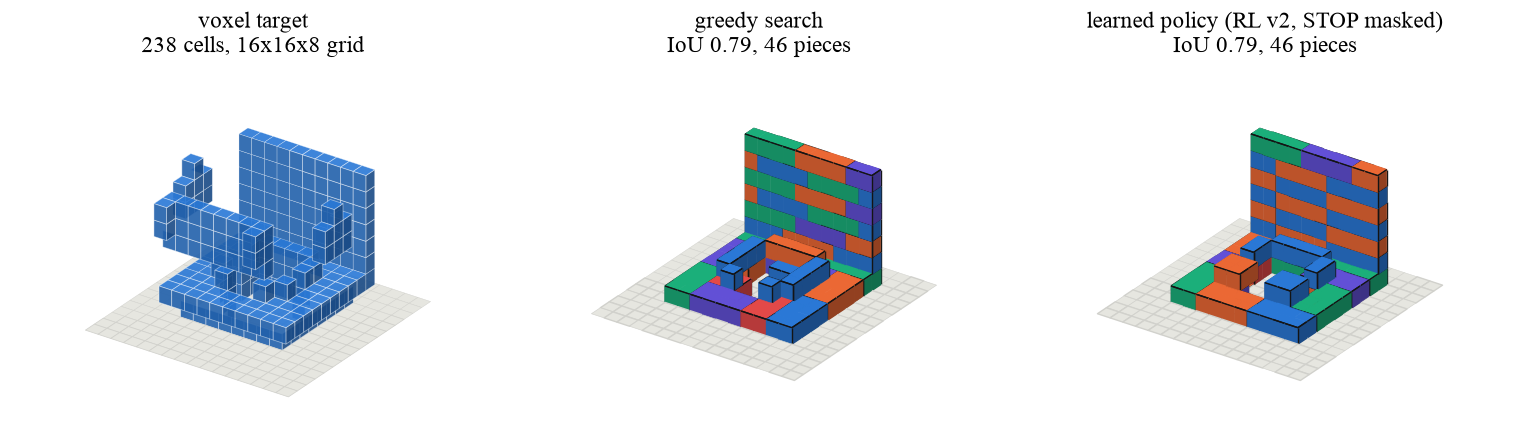
\includegraphics[width=\linewidth]{teaser}
  \caption{The task. A Thingi10K mesh is voxelized onto a 16\,$\times$\,16\,$\times$\,8 grid (left) and rebuilt from
  six kinds of brick under a 200-piece budget by the hand-written greedy search (middle) and by the learned policy
  after reinforcement learning (right). Both builds pass the same validator and assembly planner. Brick colours are
  only there to separate neighbouring pieces.}
  \label{fig:teaser}
\end{figure}

The problem is interesting because it is \emph{discrete} and \emph{constrained}. Each decision is a choice among
hundreds of legal placements, a wrong choice can block a cell forever, and whether the final structure is one
connected piece or several loose islands only becomes clear at the end. Classical approaches search this space with
hand-written heuristics. A natural question is whether a small learned policy can do as well, and whether the extra
signal available from the finished build (its fidelity, its connectedness) can be used to train that policy beyond
imitation. A second, practical question is how fidelity depends on the piece budget: a 50-piece model is cheaper to
buy and faster to build than a 200-piece one, and a designer needs to know what is lost.

We answer both questions inside one controlled pipeline. The pipeline fixes the grid (16 studs by 16 studs by 8 brick
layers), the catalogue (six basic bricks), the legality rules, the trim that keeps the largest ground-connected
component, the assembly planner, the validator and a simplified static stability check. Three generators are swapped
in and out of that pipeline:
\begin{itemize}
  \item a \textbf{greedy search} that tiles each layer bottom-up, covering the most constrained cells first;
  \item a \textbf{learned policy}, a 3D convolutional network with about 100k parameters that scores every legal
  placement plus a stop action, trained by \emph{supervised fine-tuning} (SFT) to imitate the search;
  \item the same policy after \textbf{reinforcement learning} (RL) with proximal policy optimisation (PPO), rewarded
  only by the fidelity and model-stability of the finished, trimmed build.
\end{itemize}
Everything is evaluated on a frozen benchmark of 53 held-out cases (13 procedural shapes and 40 Creative Commons
meshes from Thingi10K) at budgets of 50, 100 and 200 pieces, with an audit that regenerates every recorded number.

\paragraph{Findings.} At the 200-piece cap the RL policy with its stop action masked scores a mean intersection-over-union
(IoU) of \meanRlVTwoNostopTwoHundred{} against \meanGreedyVOneTwoHundred{} for the search; it ties the search on procedural shapes
(\meanRlVTwoNostopProc{} vs \meanGreedyVOneProc{}), trails it by 0.015 on real meshes, matches its validity (\validRlVTwoNostop/53) and
model-stability (\stableRlVTwoNostop/53) counts, and decodes in about twice the search's time, both under 0.2\,s per shape.
Its head-to-head record against the search (wins / losses / ties) is \hhRlVTwoNostopVsGreedyVOne; the median case is a tie
and the gap sits in a handful of real meshes. A second training seed reproduces the number exactly. Each stage of the ladder earned its
place: rebalancing the training data towards real meshes moved SFT from \meanSftVOneTwoHundred{} to \famSftVTwoTwoHundred{} (two-seed mean),
RL on top added between 0.02 and 0.04 over its own initialisation in both seeds, and masking the stop action
added another 0.02 to 0.03. Fidelity rises steeply from 50 to 100 pieces and barely from 100 to 200, for every
generator, because the greedy and the policy both stop when no supported placement remains rather than at the cap.

\paragraph{What did not work.} We report three negative results. The learned stop action remains miscalibrated on
real meshes after RL: with its own stop the policy ends some builds at zero pieces, and masking the action gains 0.03
to 0.09 IoU on a held-out split. The stability bonus in the reward turned out to be redundant: without it the builds
are exactly as stable (under the model) because the legality rules and the trim already enforce what the bonus
rewards. And the connectivity inputs added for RL help wherever the policy has to judge on its own (its own stop
decision, the larger held-out split) but are invisible in the benchmark mean once stop is masked and the trim cleans
up after decoding.

\paragraph{Contributions.}
\begin{enumerate}
  \item A reproducible, audited piece-budget benchmark for brick building with full failure accounting (every case
  reported, failed builds scored zero).
  \item A controlled ladder, greedy $\rightarrow$ SFT $\rightarrow$ SFT+RL on two datasets and two seeds, that
  isolates the effects of data, reinforcement learning and the decode rule.
  \item Evidence that a 100k-parameter candidate-scoring policy trained in under five hours on a laptop reaches within
  0.012 mean IoU of a hand-engineered search at comparable decode cost.
  \item Three negative results about stop calibration, reward shaping and input features, each with the evidence that
  would have been needed to claim the opposite.
\end{enumerate}

\section{Problem setup and the shared pipeline}
\label{sec:setup}

\paragraph{Grid and bricks.} A brick model lives on an integer grid. The horizontal unit is one \emph{stud}
(8\,mm pitch); the vertical unit is one \emph{plate} (3.2\,mm), and a standard brick is three plates tall. We use a
16\,$\times$\,16 stud footprint and 8 brick layers, which is 2048 cells of one stud by one stud by one brick. The
catalogue has six upright bricks: 1\,$\times$\,1, 1\,$\times$\,2, 1\,$\times$\,3, 1\,$\times$\,4, 2\,$\times$\,2 and
2\,$\times$\,4, placed at 0\textdegree{} or 90\textdegree. A \emph{placement} is a brick type, rotation and
position; a \emph{build} is a list of placements plus an ordered list of assembly steps.

\paragraph{Target.} The input is a watertight mesh. It is rotated so its chosen axis points up, scaled uniformly to fit
the physical box the grid represents, floored, and voxelized by testing whether each cell centre lies inside the
mesh. The result is a boolean \emph{target} grid $T$. (Procedural targets are generated directly on the grid.)

\paragraph{Legality.} A placement is legal when it lies inside the grid, overlaps no placed brick, is \emph{supported}
(it sits on the ground or at least one cell directly beneath it is already filled), covers at least one target cell,
and is at most half \emph{filler}, cells outside the target. These rules are enforced by a candidate enumerator that
every generator in this paper shares, so no generator can place an illegal brick.

\paragraph{The finalize step.} Every generator returns a raw list of placements, and every list goes through the
same four stages (Figure~\ref{fig:pipeline}):
\begin{enumerate}
  \item \textbf{Trim.} Bricks connect only through studs: an upper brick is attached to a lower one when it rests
  directly on it with overlapping footprints. Side contact does not count. The build is reduced to its largest
  component connected to the ground; everything else is discarded. This is what makes the output one object.
  \item \textbf{Plan.} A planner orders the remaining bricks one per step, each inserted straight down, attached to
  what is already there, with a clear insertion path and never sealing an unplaced brick beneath it. For this
  catalogue of same-height upright bricks that greedy planner is complete: every valid build gets an order.
  \item \textbf{Validate.} An independent validator replays the steps and checks bounds, collisions, support, the
  single-component property and the piece budget. A build that fails here is reported as invalid.
  \item \textbf{Stability check.} A linear simplification of the StableLego force model~\citep{liu2024stablelego}: bricks
  are rigid, loaded by their own weight; each shared stud cell carries vertical force at four points; compression is
  unbounded and tension is capped by a clutch capacity of 0.98\,N per stud cell, divided over its four points. The
  constant is StableLego's measured value, which that work applies per contact point rather than per stud, so our
  limit is roughly four times more conservative than theirs. A linear program
  finds the smallest tension utilisation that balances every brick. Utilisation at most one is \emph{stable under the
  model}. The model ignores lateral loads, friction and deformation, so throughout this paper ``stable'' means
  \stablenote.
\end{enumerate}

\begin{figure}[t]
  \centering
  \resizebox{\linewidth}{!}{%
  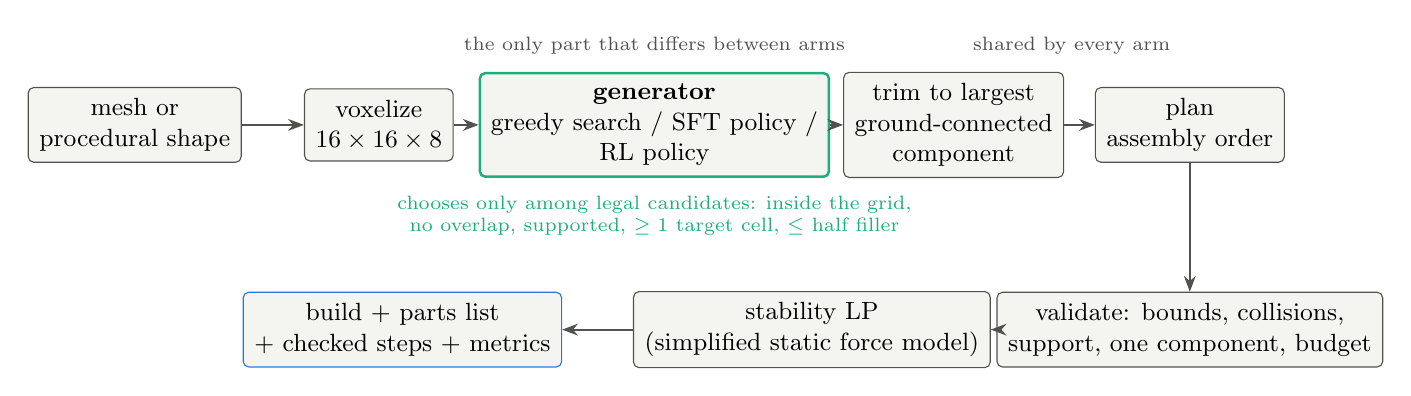
\begin{tikzpicture}[
    box/.style={draw=muted, fill=boxc, rounded corners=2pt, align=center, font=\small, minimum height=9mm, inner sep=4pt},
    gen/.style={box, draw=rlc, line width=0.9pt},
    arr/.style={-{Stealth[length=2mm]}, muted, line width=0.7pt},
    lab/.style={font=\scriptsize, text=muted, align=center}]
    \node[box] (mesh) at (0,0) {mesh or\\procedural shape};
    \node[box] (vox) at (3.1,0) {voxelize\\$16\times16\times8$};
    \node[gen] (gen) at (6.6,0) {\textbf{generator}\\greedy search / SFT policy /\\RL policy};
    \node[box] (trim) at (10.4,0) {trim to largest\\ground-connected\\component};
    \node[box] (plan) at (13.4,0) {plan\\assembly order};
    \node[box] (val) at (13.4,-2.6) {validate: bounds, collisions,\\support, one component, budget};
    \node[box] (stab) at (8.6,-2.6) {stability LP\\(simplified static force model)};
    \node[box, draw=greedyc] (out) at (3.4,-2.6) {build + parts list\\+ checked steps + metrics};
    \draw[arr] (mesh) -- (vox);
    \draw[arr] (vox) -- (gen);
    \draw[arr] (gen) -- (trim);
    \draw[arr] (trim) -- (plan);
    \draw[arr] (plan) -- (val);
    \draw[arr] (val) -- (stab);
    \draw[arr] (stab) -- (out);
    \node[lab, above=1mm of gen] {the only part that differs between arms};
    \node[lab, above=1mm of trim, xshift=1.5cm] {shared by every arm};
    \node[lab, below=1mm of gen, text=rlc] {chooses only among legal candidates: inside the grid,\\no overlap, supported, $\geq 1$ target cell, $\leq$ half filler};
  \end{tikzpicture}}
  \caption{The shared pipeline. Generators differ only in how they choose the next brick; the trim, planner,
  validator and stability check are identical, so fidelity differences cannot come from different rules.}
  \label{fig:pipeline}
\end{figure}

\paragraph{Metrics.} \emph{Fidelity} is the intersection-over-union between the occupancy of the trimmed build $B$ and
the target, $\iou = |B \cap T| / |B \cup T|$, so both missing and extraneous cells count. \emph{Validity} is the
validator's verdict, \emph{stability} the force model's, \emph{pieces} the brick count after the trim, and
\emph{decode time} the wall-clock seconds the generator took. The \emph{piece budget} is a hard cap on placements;
a generator may stop earlier.

\paragraph{Fidelity convention.} Throughout, a reported mean IoU is the mean over the \nAttempted{} benchmark cases
that are attemptable (one fixture is a deliberately non-watertight mesh that every generator must reject), with a
build that is missing or fails validation scored 0. A generator therefore cannot raise its mean by failing on hard
cases. The benchmark's own summariser averages over valid builds only, which reads higher for generators with
failures; we never use that number for comparisons.

\section{Three ways to choose the next brick}
\label{sec:generators}

\subsection{Greedy search (the baseline and the teacher)}
The baseline builds layer by layer from the ground up. Within a layer it repeatedly scores every legal placement of
every brick type and takes the best. The score puts \emph{hard} cells first: a target cell with nothing beneath it can
only ever be covered by a brick that also overlaps the layer below, so the search covers those before they become
unreachable. After hard cells it prefers placements that cover more new target cells, then fewer filler cells, then
more support underneath; ties break on the number of distinct bricks below (to interlock), part cost and position.
Three filler policies (none, at most a quarter, at most half) are run and the best validated IoU is kept. The whole
search takes 0.07\,s per shape on average. Its output, ordered by the planner, is also the \emph{teacher} that the
learned policy imitates.

\subsection{The policy network}
The learned generator is a candidate-scoring network (Figure~\ref{fig:policy}). Its input is the grid as three
voxel channels (target, current assembly, remaining target), encoded by four 3D convolutions with 32 channels at
full resolution (the grid is small enough that no pooling is needed). For each legal placement the encoder's features
are averaged over the placement's footprint cells and concatenated with 13 hand-computed features (the brick type as
a one-hot code, rotation, position, and the counts of new target, filler and supporting cells); a small MLP turns that
into one logit. A separate head scores the \emph{stop} action from a global pool of the feature map. A softmax over
all candidates plus stop gives the policy. Because only enumerated legal placements receive logits, legality is
inherent at training and at inference. The policy has 97k parameters; RL adds a value head and two inputs described
below, for 101k in total.

\begin{figure}[t]
  \centering
  \resizebox{\linewidth}{!}{%
  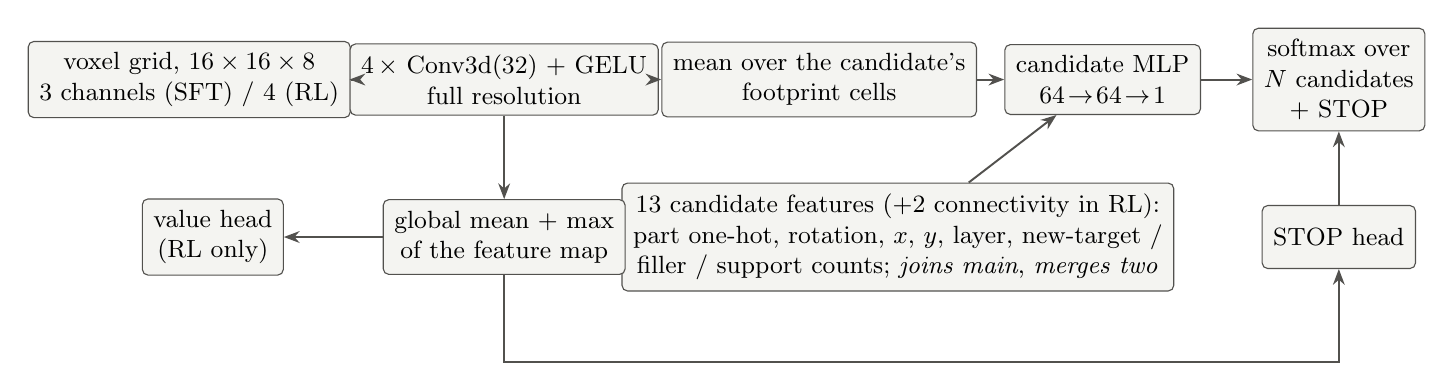
\begin{tikzpicture}[
    box/.style={draw=muted, fill=boxc, rounded corners=2pt, align=center, font=\small, inner sep=4pt, minimum height=8mm},
    arr/.style={-{Stealth[length=2mm]}, muted, line width=0.7pt},
    lab/.style={font=\scriptsize, text=muted, align=center}]
    \node[box] (vox) at (0,0) {voxel grid, $16\times16\times8$\\3 channels (SFT) / 4 (RL)};
    \node[box] (enc) at (4.0,0) {4\,$\times$ Conv3d(32) + GELU\\full resolution};
    \node[box] (pool) at (8.0,0) {mean over the candidate's\\footprint cells};
    \node[box] (mlp) at (11.6,0) {candidate MLP\\$64\!\to\!64\!\to\!1$};
    \node[box] (soft) at (14.6,0) {softmax over\\$N$ candidates\\+ STOP};
    \node[box] (feat) at (9.0,-2.0) {13 candidate features (+2 connectivity in RL):\\part one-hot, rotation, $x$, $y$, layer, new-target /\\filler / support counts; \emph{joins main}, \emph{merges two}};
    \node[box] (glob) at (4.0,-2.0) {global mean + max\\of the feature map};
    \node[box] (val) at (0.3,-2.0) {value head\\(RL only)};
    \node[box] (stop) at (14.6,-2.0) {STOP head};
    \draw[arr] (vox) -- (enc);
    \draw[arr] (enc) -- (pool);
    \draw[arr] (pool) -- (mlp);
    \draw[arr] (feat) -- (mlp);
    \draw[arr] (mlp) -- (soft);
    \draw[arr] (enc) -- (glob);
    \draw[arr] (glob) -- (val);
    \draw[arr] (glob.south) -- ++(0,-1.1) -| (stop.south);
    \draw[arr] (stop) -- (soft);
  \end{tikzpicture}}
  \caption{The candidate-scoring policy. Every legal placement is scored from pooled voxel features and a few
  hand-computed counts; STOP is scored from a global pool. 97k parameters (101k with the RL value head and
  connectivity inputs).}
  \label{fig:policy}
\end{figure}

\subsection{Imitation (SFT)}
\paragraph{Data.} Targets come from two sources. Ten procedural families (boxes, stacks, capped towers, bridges,
polyominoes, ellipsoids, cylinders, stepped shapes, blobs, rows of arches), 200 instances each, grounded and
face-connected. And a pool of Thingi10K meshes with every benchmark object excluded, voxelized by the production
pipeline. The supervision for each target is the greedy search's validated build in planner order, ending with the
stop action. We trained on two versions of this pool. \textbf{v1} kept 150 real meshes (at most 50k faces, and only
those on which the teacher covered at least half the target), so training was 93\,\% procedural. \textbf{v2} kept
every eligible mesh, 640 real meshes up to 200k faces, and draws half of each training batch from them. Examples
are split 80/10/10 by object, with all symmetric copies and all files of one Thingiverse object in the same split.

\paragraph{Training.} Teacher forcing with cross-entropy over candidates plus stop; AdamW at $10^{-3}$ with a cosine
schedule, batch 32, 20{,}000 steps, 8-fold symmetry augmentation (rotations and reflections of the grid). Decisions
are streamed by a background producer because materialising every augmented decision would need about 40\,GB.
Checkpoints are selected by free-running decode IoU on a fixed validation subset, not by teacher-forced accuracy,
because the latter hides compounding errors. One run takes 25 to 28 minutes on the laptop's GPU.

\subsection{Reinforcement learning}
Imitation reproduces the teacher's per-step choices but cannot see what only shows up in the finished build: whether
the layers interlock into one component, or whether an early placement blocked a cell for good. RL scores the
finished build directly.

\paragraph{Environment.} An episode places bricks on one target with the same candidate set plus stop, under
temperature-1 sampling. The state tracks a union-find over stud connections so the \emph{main} (largest grounded)
component is known at every step, exactly as the trim will decide it. Two things are added to the observation: a
fourth voxel channel marking the main component, and two per-candidate features, \emph{joins the main component} and
\emph{merges two components}. The SFT weights are zero-padded into this layout, so the initial RL policy produces the
SFT policy's logits exactly. The terminal reward is computed after the shared finalize step:
\[
  r \;=\; \iou_{\text{after trim}} \;+\; 0.1\cdot[\text{stable under the model}],
\]
with no per-step shaping. Validity cannot fail under the candidate rules, so no penalty is needed.

\paragraph{Algorithm.} PPO~\citep{schulman2017ppo} with a value head on the same encoder; advantage is reward minus
value (terminal reward only), normalised per batch; clip 0.2, entropy bonus 0.01, a KL penalty of 0.05 towards the
frozen initial policy, Adam at $10^{-4}$, gradient clipping 1.0. Masked actions are removed from the entropy and KL
terms before any multiplication; leaving them in poisons the backward pass with NaNs. Each iteration samples 128
episodes in 8 forked CPU workers and runs 3 epochs of updates on the GPU; 250 iterations take 1.6 to 2.4 hours. The
best checkpoint is chosen by greedy-decode IoU on a fixed 64-example validation subset that mirrors the training mix
(half real meshes in v2).

\paragraph{Decode rule.} At inference the policy decodes greedily (argmax). The stop action can be used as learned,
or \emph{masked}, in which case decoding continues until no legal placement remains or the cap is reached, exactly as
the greedy search stops. Section~\ref{sec:benchmark} describes how this choice was made.

\section{Benchmark and protocol}
\label{sec:benchmark}

\paragraph{The suite.} \nCases{} cases were frozen before any learned generator existed. Thirteen are procedural
fixtures with known expected behaviour: simple solids (cube, slab, tower, L and T shapes, wedge), overhangs (pyramid,
sphere), a budget-limited cylinder, a bridge, and three adversarial inputs (a flat sheet that cannot be covered, a
one-cell pole that admits no valid build, and a non-watertight mesh that must be rejected). Forty are Thingi10K
meshes~\citep{zhou2016thingi10k}, drawn deterministically from the models that are Creative Commons licensed and are
closed, manifold, single-component solids with 100 to 200k faces, one file per Thingiverse object. The 40 meshes
are the held-out set: every Thingiverse object in the benchmark is excluded from every training pool, and the
procedural fixtures are hand-made shapes distinct from the ten training families. Licence, author and source link are
recorded per mesh.

\paragraph{Records and audit.} Every (case, generator, budget) triple produces one record with status, fidelity,
coverage, piece count, validity, planning outcome, stability verdict, per-stage seconds, hardware and git commit.
An \emph{audit} command regenerates every non-failed record from scratch, validates it with the independent
validator, recomputes IoU from occupancy and compares status, pieces, validity and IoU with what the file claims. Every
benchmark file in this paper passed its audit, and the greedy rows are byte-identical to the frozen baseline file in
every run. The audit earned its keep once: it exposed that one mesh voxelized to 288, 289 or 290 cells depending on
the process, because the containment test re-checks ambiguous cell centres with a ray direction drawn from the global
random generator. Voxelization now runs that test under a fixed, restored random state.

\paragraph{Budgets, seeds, cost.} Every generator runs at budgets of 50, 100 and 200 pieces. Decode is deterministic
(greedy), so the benchmark seed only matters for provenance; \emph{training} seeds are reported separately
(Section~\ref{sec:seeds}). Decode time is recorded per case on the same machine for every generator.

\paragraph{Decisions were made off the benchmark.} The one decode choice for the learned generators, whether to use
the learned stop or to mask it, was made on the SFT \emph{test split} (260 held-out training-distribution examples,
188 procedural and 72 real), before any benchmark run of the affected checkpoint, and is reported in full in
Section~\ref{sec:stop}. The benchmark was never used to select a checkpoint, a decode rule or a hyperparameter.

\section{Results}
\label{sec:results}

Table~\ref{tab:main} gives the main numbers and Figure~\ref{fig:budget} the budget curves. We first read off the
budget study, then the comparison between the learned policies and the search, then the ladder that attributes the
gain, then seeds, ablations and failure analysis.

\begin{table}[t]
  \centering\small
  \caption{Mean IoU after trim over the \nAttempted{} attempted cases (failed builds scored 0) at each piece budget,
  with the split at the 200-piece cap, validity and model-stability counts out of 53, and mean decode seconds per
  case. SFT and RL v2 are the mean of two training seeds. STOP masked: decoding continues until no legal placement
  remains. Stable means \stablenote.}
  \label{tab:main}
  \footnotesize\setlength{\tabcolsep}{3.5pt}
  \begin{tabular}{llcccccccc}
    \toprule
    generator & data & 50 & 100 & 200 & procedural & Thingi10K & valid & stable & s/case \\
    \midrule
    greedy search (frozen baseline) & -- & \meanGreedyVOneFifty & \meanGreedyVOneHundred & \textbf{\meanGreedyVOneTwoHundred} & \meanGreedyVOneProc & \textbf{\meanGreedyVOneReal} & \validGreedyVOne & \stableGreedyVOne & \secsGreedyVOne \\
    \midrule
    SFT & v1 & \meanSftVOneFifty & \meanSftVOneHundred & \meanSftVOneTwoHundred & \meanSftVOneProc & \meanSftVOneReal & \validSftVOne & \stableSftVOne & \secsSftVOne \\
    SFT + RL & v1 & \meanRlVOneFifty & \meanRlVOneHundred & \meanRlVOneTwoHundred & \meanRlVOneProc & \meanRlVOneReal & \validRlVOne & \stableRlVOne & \secsRlVOne \\
    SFT + RL, STOP masked & v1 & \meanRlVOneNostopFifty & \meanRlVOneNostopHundred & \meanRlVOneNostopTwoHundred & \meanRlVOneNostopProc & \meanRlVOneNostopReal & \validRlVOneNostop & \stableRlVOneNostop & \secsRlVOneNostop \\
    \midrule
    SFT (2 s.) & v2 & \famSftVTwoFifty & \famSftVTwoHundred & \famSftVTwoTwoHundred & \meanSftVTwoProc & \meanSftVTwoReal & \validSftVTwo & \stableSftVTwo & \secsSftVTwo \\
    SFT + RL (2 s.) & v2 & \famRlVTwoFifty & \famRlVTwoHundred & \famRlVTwoTwoHundred & \meanRlVTwoProc & \meanRlVTwoReal & \validRlVTwo & \stableRlVTwo & \secsRlVTwo \\
    SFT + RL, STOP masked (2 s.) & v2 & \famRlVTwoNostopFifty & \famRlVTwoNostopHundred & \textbf{\famRlVTwoNostopTwoHundred} & \meanRlVTwoNostopProc & \meanRlVTwoNostopReal & \validRlVTwoNostop & \stableRlVTwoNostop & \secsRlVTwoNostop \\
    \bottomrule
  \end{tabular}
  \par\smallskip\footnotesize The split, validity, stability and time columns for the v2 rows are seed 0; seed 1 is
  in Table~\ref{tab:seeds}.
\end{table}

\begin{figure}[t]
  \centering
  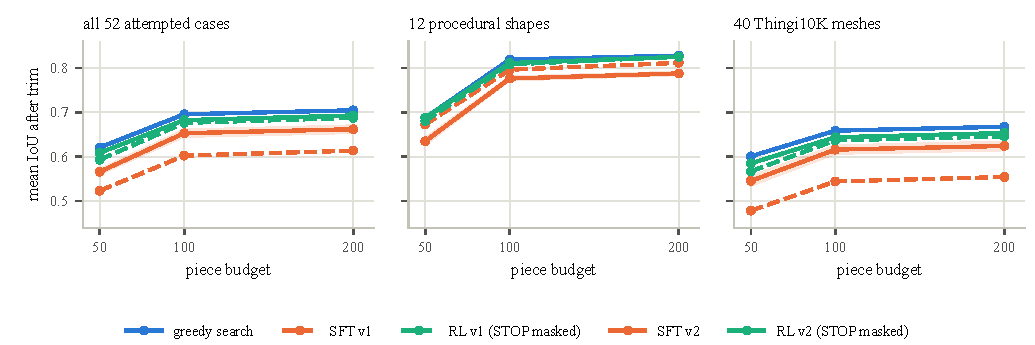
\includegraphics[width=\linewidth]{budget}
  \caption{Fidelity against piece budget for the search (blue), imitation (orange) and reinforcement learning
  (green) on the v1 data (dashed) and the v2 data (solid). Bands are the range over two training seeds. Every arm
  gains most between 50 and 100 pieces and little between 100 and 200, because the cap rarely binds: the mean build
  has about 39 pieces at the 200 cap.}
  \label{fig:budget}
\end{figure}

\subsection{Piece budget versus fidelity}
Fidelity is a concave function of the budget for every generator (Figure~\ref{fig:budget}). From 50 to 100 pieces the
search gains 0.075 and the best learned arm 0.074; from 100 to 200 they gain 0.009 and 0.012. The reason is visible in
the records: at the 200 cap the mean build has about 39 pieces and the cap is the stopping reason for almost no
case. Both the search and the policy stop when no supported, non-overlapping placement that covers a target cell
remains, which for these shapes happens long before 200 bricks. Fifty pieces, by contrast, truncates most real
meshes mid-build. The practical reading for a designer is that on this grid a 100-piece budget buys nearly all the
fidelity that 200 does. The ordering of the arms is the same at every budget, so the comparison below is reported at
200 without loss.

\subsection{Learned policy versus hand-written search}
\begin{figure}[t]
  \centering
  \begin{minipage}[t]{0.48\linewidth}
    \centering
    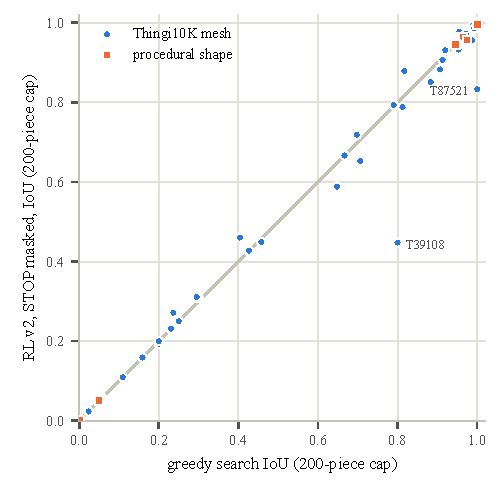
\includegraphics[width=\linewidth]{scatter}
    \caption{Per-case fidelity at the 200-piece cap, RL v2 with STOP masked against the greedy search. Most cases
    lie on the diagonal; the head-to-head record (wins / losses / ties) is \hhRlVTwoNostopVsGreedyVOne. The honeycomb
    pot T39108 is the one large loss.}
    \label{fig:scatter}
  \end{minipage}\hfill
  \begin{minipage}[t]{0.48\linewidth}
    \centering
    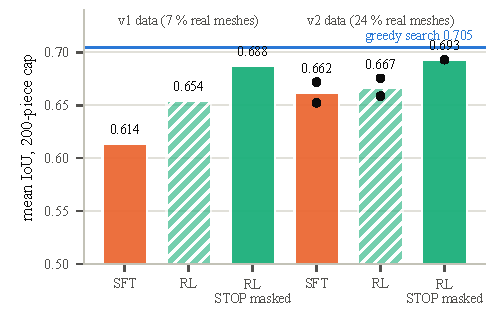
\includegraphics[width=\linewidth]{ladder}
    \caption{The ladder at the 200-piece cap. Hatched bars use the learned STOP; dots are the two training seeds of
    the v2 arms. Rebalancing the data moved SFT up, RL added more, and masking STOP added the rest.}
    \label{fig:ladder}
  \end{minipage}
\end{figure}

The RL v2 policy with STOP masked is within 0.012 mean IoU of the search at every budget. On the 12 procedural shapes
it ties (\meanRlVTwoNostopProc{} vs \meanGreedyVOneProc); on the 40 real meshes it trails by 0.015 (\meanRlVTwoNostopReal{} vs
\meanGreedyVOneReal). Its validity count (\validRlVTwoNostop/53) and model-stability count (\stableRlVTwoNostop/53) equal the
search's; the two invalid cases are the adversarial fixtures that no generator can build, so 51 is the ceiling. It
decodes in \secsRlVTwoNostop\,s per case against the search's \secsGreedyVOne\,s. Figure~\ref{fig:scatter} shows the per-case
picture: the median case is a tie, the head-to-head record is \hhRlVTwoNostopVsGreedyVOne{} (wins / losses / ties), and the
remaining gap sits in a handful of real meshes, one of which (a honeycomb pot, Section~\ref{sec:failures}) accounts for most of it.

Two comparisons bound what this means. Against its own SFT initialisation the RL policy's record is
\hhRlVTwoNostopVsSftVTwo{} (seed 0) and \hhRlVTwoSOneNostopVsSftVTwoSOne{} (seed 1). Against a test-time-compute baseline, best-of-8 sampling
from the v1 SFT policy at about seven times the decode cost, the single-sample RL v1 policy with STOP masked scores
\meanRlVOneNostopTwoHundred{} against 0.686: RL's advantage over sampling is cost, not ceiling.

\subsection{What produced the gain: data, RL, decode rule}
\label{sec:ladder}
Figure~\ref{fig:ladder} separates the three changes between the first learned arm and the last.
\begin{itemize}
  \item \textbf{Data.} The same SFT recipe on the v2 pool, which has four times as many real meshes and draws half of
  each batch from them, moves SFT from \meanSftVOneTwoHundred{} to \famSftVTwoTwoHundred{} (mean of two seeds, range
  \famloSftVTwoTwoHundred--\famhiSftVTwoTwoHundred). Given the 0.02 spread between seeds at the SFT stage, we state this gain as +0.04 to +0.06.
  \item \textbf{RL.} On the v1 data RL adds +0.040 over SFT with the learned stop (\meanSftVOneTwoHundred{} $\to$ \meanRlVOneTwoHundred).
  On the v2 data, with STOP masked, RL adds +0.021 to seed 0 and +0.041 to seed 1, and both seeds land on
  \famRlVTwoNostopTwoHundred. RL beats its own initialisation 26 to 3 and 27 to 9 head to head. Where the gain comes from is
  shown by the diagnostic fields: on the v1 ladder, fragmented builds fall from 27 to 22 of 52 and the mean number of
  pieces removed by the trim falls from 6.0 to 3.2. Figure~\ref{fig:curves} shows the training curves: validation IoU
  rises from the SFT value to within 0.02 of the teacher on the same subset, fragmentation roughly halves, and policy
  entropy stays near 1.3 to 1.6 nats with the KL to the initial policy around 0.2 to 0.3, so the policy moved without
  collapsing.
  \item \textbf{Decode rule.} Masking the learned stop adds +0.034 to RL v1 and +0.034 (seed 0) / +0.018 (seed 1) to
  RL v2. One caveat belongs here: with its \emph{own} stop, RL v2 (\meanRlVTwoTwoHundred) is below SFT v2
  (\meanSftVTwoTwoHundred) on the mean, because the RL policy stops at zero pieces on a few real meshes; the RL gain is
  only realised once stop is masked (Section~\ref{sec:stop}).
\end{itemize}

\begin{figure}[t]
  \centering
  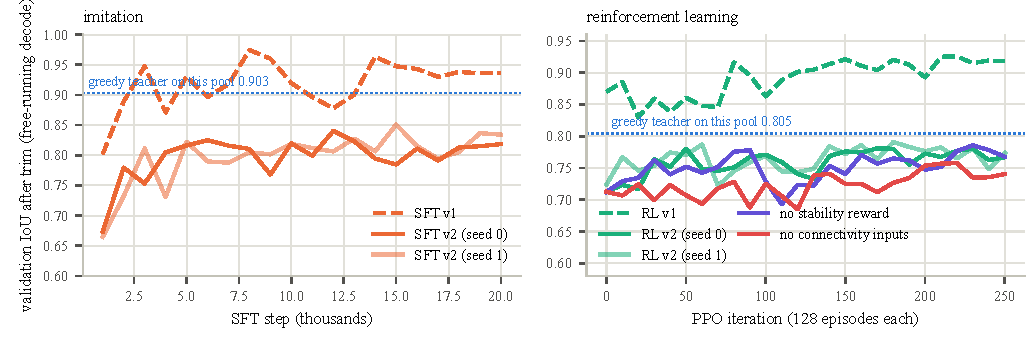
\includegraphics[width=\linewidth]{curves}
  \caption{Training curves. Left: free-running validation IoU during imitation (every 1000 steps); the v1 pool is
  almost entirely procedural and its teacher reaches 0.903 on it, the v2 pool is half real meshes and harder. Right:
  validation IoU during PPO (every 10 iterations) for both v2 seeds, the v1 run and the two ablations; the dotted
  lines are the greedy teacher on the same validation subsets.}
  \label{fig:curves}
\end{figure}

\subsection{Two training seeds}
\label{sec:seeds}
Every arm of the v2 ladder was retrained end to end with a second seed (Table~\ref{tab:seeds}). The headline reproduces:
RL v2 with STOP masked scores \famloRlVTwoNostopTwoHundred{} and \famhiRlVTwoNostopTwoHundred{} at the 200 cap, 0.012 behind the search either
way, and wins 10 and 11 cases against it. The per-case picture is also stable: the same 12 cases are lost to the search
in both seeds and the same 6 real meshes are won in both. The one count where seed 1 is worse is stability, 47
against 49 stable builds at the 200 cap (validity is identical at 51). The SFT stage, by contrast, differs by 0.020
between seeds; RL removes that spread. Two seeds give a range, not a confidence interval, and we report both numbers
rather than a mean with an error bar.

\begin{table}[t]
  \centering\small
  \caption{The v2 ladder for both training seeds at the 200-piece cap (mean IoU over attempted cases; wins / losses /
  ties against the search). The v1 arms and the ablations are single-seed.}
  \label{tab:seeds}
  \footnotesize\setlength{\tabcolsep}{3pt}
  \begin{tabular}{lccccccc}
    \toprule
    arm & s0 & s1 & procedural s0 / s1 & Thingi10K s0 / s1 & valid & stable & vs search s0; s1 \\
    \midrule
    SFT v2 & \meanSftVTwoTwoHundred & \meanSftVTwoSOneTwoHundred & \meanSftVTwoProc{} / \meanSftVTwoSOneProc & \meanSftVTwoReal{} / \meanSftVTwoSOneReal & \validSftVTwo{} / \validSftVTwoSOne & \stableSftVTwo{} / \stableSftVTwoSOne & \hhSftVTwoVsGreedyVOne; 4 / 28 / 20 \\
    RL v2 (learned STOP) & \meanRlVTwoTwoHundred & \meanRlVTwoSOneTwoHundred & \meanRlVTwoProc{} / \meanRlVTwoSOneProc & \meanRlVTwoReal{} / \meanRlVTwoSOneReal & \validRlVTwo{} / \validRlVTwoSOne & \stableRlVTwo{} / \stableRlVTwoSOne & 7 / 27 / 18; 7 / 25 / 20 \\
    RL v2, STOP masked & \meanRlVTwoNostopTwoHundred & \meanRlVTwoSOneNostopTwoHundred & \meanRlVTwoNostopProc{} / \meanRlVTwoSOneNostopProc & \meanRlVTwoNostopReal{} / \meanRlVTwoSOneNostopReal & \validRlVTwoNostop{} / \validRlVTwoSOneNostop & \stableRlVTwoNostop{} / \stableRlVTwoSOneNostop & \hhRlVTwoNostopVsGreedyVOne; \hhRlVTwoSOneNostopVsGreedyVOne \\
    \bottomrule
  \end{tabular}
\end{table}

\subsection{The stop action}
\label{sec:stop}
Table~\ref{tab:stop} (Appendix~\ref{app:stop}) is the decision table, computed on the SFT test split before each
checkpoint touched the benchmark. Masking the stop action never costs anything on procedural shapes and gains 0.03 to 0.09 on real meshes for
all five RL checkpoints (two seeds, two ablations, and v1), so the masked decode is the one reported for each. On the
benchmark the learned stop is the cause of every zero-piece build: the policy stops before placing anything on three
to six real meshes per checkpoint, different meshes for different seeds (seed 0: four meshes; seed 1: three; only one
in common). Figure~\ref{fig:stops} shows how builds end. Our reading is that the policy learned that on shapes where
every remaining candidate looks poor, stopping has the highest expected value under its own future behaviour, even
though the terminal reward penalises exactly that and half the RL episodes were real meshes. Masked decoding forces
the policy to keep tiling and lets the trim keep the largest connected part; it fragments more often (25 of 40 real
builds have pieces removed by the trim, against 14 with the learned stop) but ends with more of the target covered.


\begin{figure}[t]
  \centering
  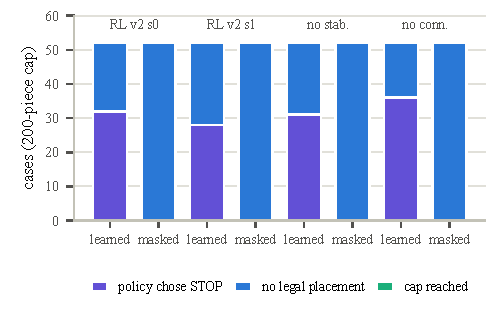
\includegraphics[width=0.6\linewidth]{stops}
  \caption{Why builds end at the 200-piece cap, for each RL checkpoint with the learned and the masked stop. The cap
  itself is never reached. With the learned stop, the policy chooses to stop on 28 to 36 of 52 cases, including a
  few at zero pieces.}
  \label{fig:stops}
\end{figure}

\subsection{Ablations}
\label{sec:ablations}
Two arms were retrained from the same seed-0 SFT checkpoint with the RL v2 settings, changing one thing each
(Table~\ref{tab:ablations}).

\begin{table}[t]
  \centering\small
  \caption{Ablations of RL v2 at the 200-piece cap (single seed; STOP masked unless stated). Wins / losses / ties are
  against the full RL v2 with STOP masked. Stable means \stablenote.}
  \label{tab:ablations}
  \begin{tabular}{lcccccc}
    \toprule
    arm & mean IoU & procedural & Thingi10K & valid & stable & vs RL v2 \\
    \midrule
    RL v2, STOP masked (reference) & \meanRlVTwoNostopTwoHundred & \meanRlVTwoNostopProc & \meanRlVTwoNostopReal & \validRlVTwoNostop & \stableRlVTwoNostop & -- \\
    no stability reward & \meanRlVTwoNostabNostopTwoHundred & \meanRlVTwoNostabNostopProc & \meanRlVTwoNostabNostopReal & \validRlVTwoNostabNostop & \stableRlVTwoNostabNostop & \hhRlVTwoNostabNostopVsRlVTwoNostop \\
    no connectivity inputs & \meanRlVTwoNoconnNostopTwoHundred & \meanRlVTwoNoconnNostopProc & \meanRlVTwoNoconnNostopReal & \validRlVTwoNoconnNostop & \stableRlVTwoNoconnNostop & \hhRlVTwoNoconnNostopVsRlVTwoNostop \\
    \midrule
    no stability reward, learned STOP & \meanRlVTwoNostabTwoHundred & \meanRlVTwoNostabProc & \meanRlVTwoNostabReal & \validRlVTwoNostab & \stableRlVTwoNostab & \\
    no connectivity inputs, learned STOP & \meanRlVTwoNoconnTwoHundred & \meanRlVTwoNoconnProc & \meanRlVTwoNoconnReal & \validRlVTwoNoconn & \stableRlVTwoNoconn & \\
    \bottomrule
  \end{tabular}
\end{table}

\paragraph{The stability reward is redundant.} With the stability term removed from the reward, the builds are
exactly as stable as with it: 147 of 153 valid builds across the three budgets, the same two real meshes unstable at
the 200 cap, identical to the search. The legality rule that every brick must rest on something, together with the
trim to one grounded component, already produces structures the force model accepts; the bonus had nothing left to
reward. Fidelity moves by 0.007 (\hhRlVTwoNostabNostopVsRlVTwoNostop{} head to head), a single-seed difference smaller than the
0.02 seed spread at the SFT stage, though one case moves a lot (the honeycomb pot falls from 0.45 to 0.25). The
clean statement is that in this setting stability comes from the hard constraints, not from reward shaping.

\paragraph{The connectivity inputs matter where the policy judges on its own.} Removing the main-component channel and
the two connectivity features costs 0.064 on the benchmark under the learned stop (\meanRlVTwoNoconnTwoHundred{} vs
\meanRlVTwoTwoHundred), with six real meshes ending at zero pieces; it costs 0.035 on the 260-example test split with stop masked
(Table~\ref{tab:stop} in Appendix~\ref{app:stop}, 0.805 vs 0.840) and 0.023 on the validation curve. Yet on the 52-case benchmark with stop
masked the means are within 0.003 (\meanRlVTwoNoconnNostopTwoHundred{} vs \meanRlVTwoNostopTwoHundred), because one large win on the honeycomb
pot (0.78 vs 0.45) offsets 18 losses to 7 wins. Head to head it is the weaker policy; the benchmark mean is too
coarse to show it. The features' main job is telling the policy which candidates attach to the main component and
when a build is finished. With stop masked, the trim does that cleanup after decoding for free.

\subsection{Failure analysis}
\label{sec:failures}
\begin{figure}[p]
  \centering
  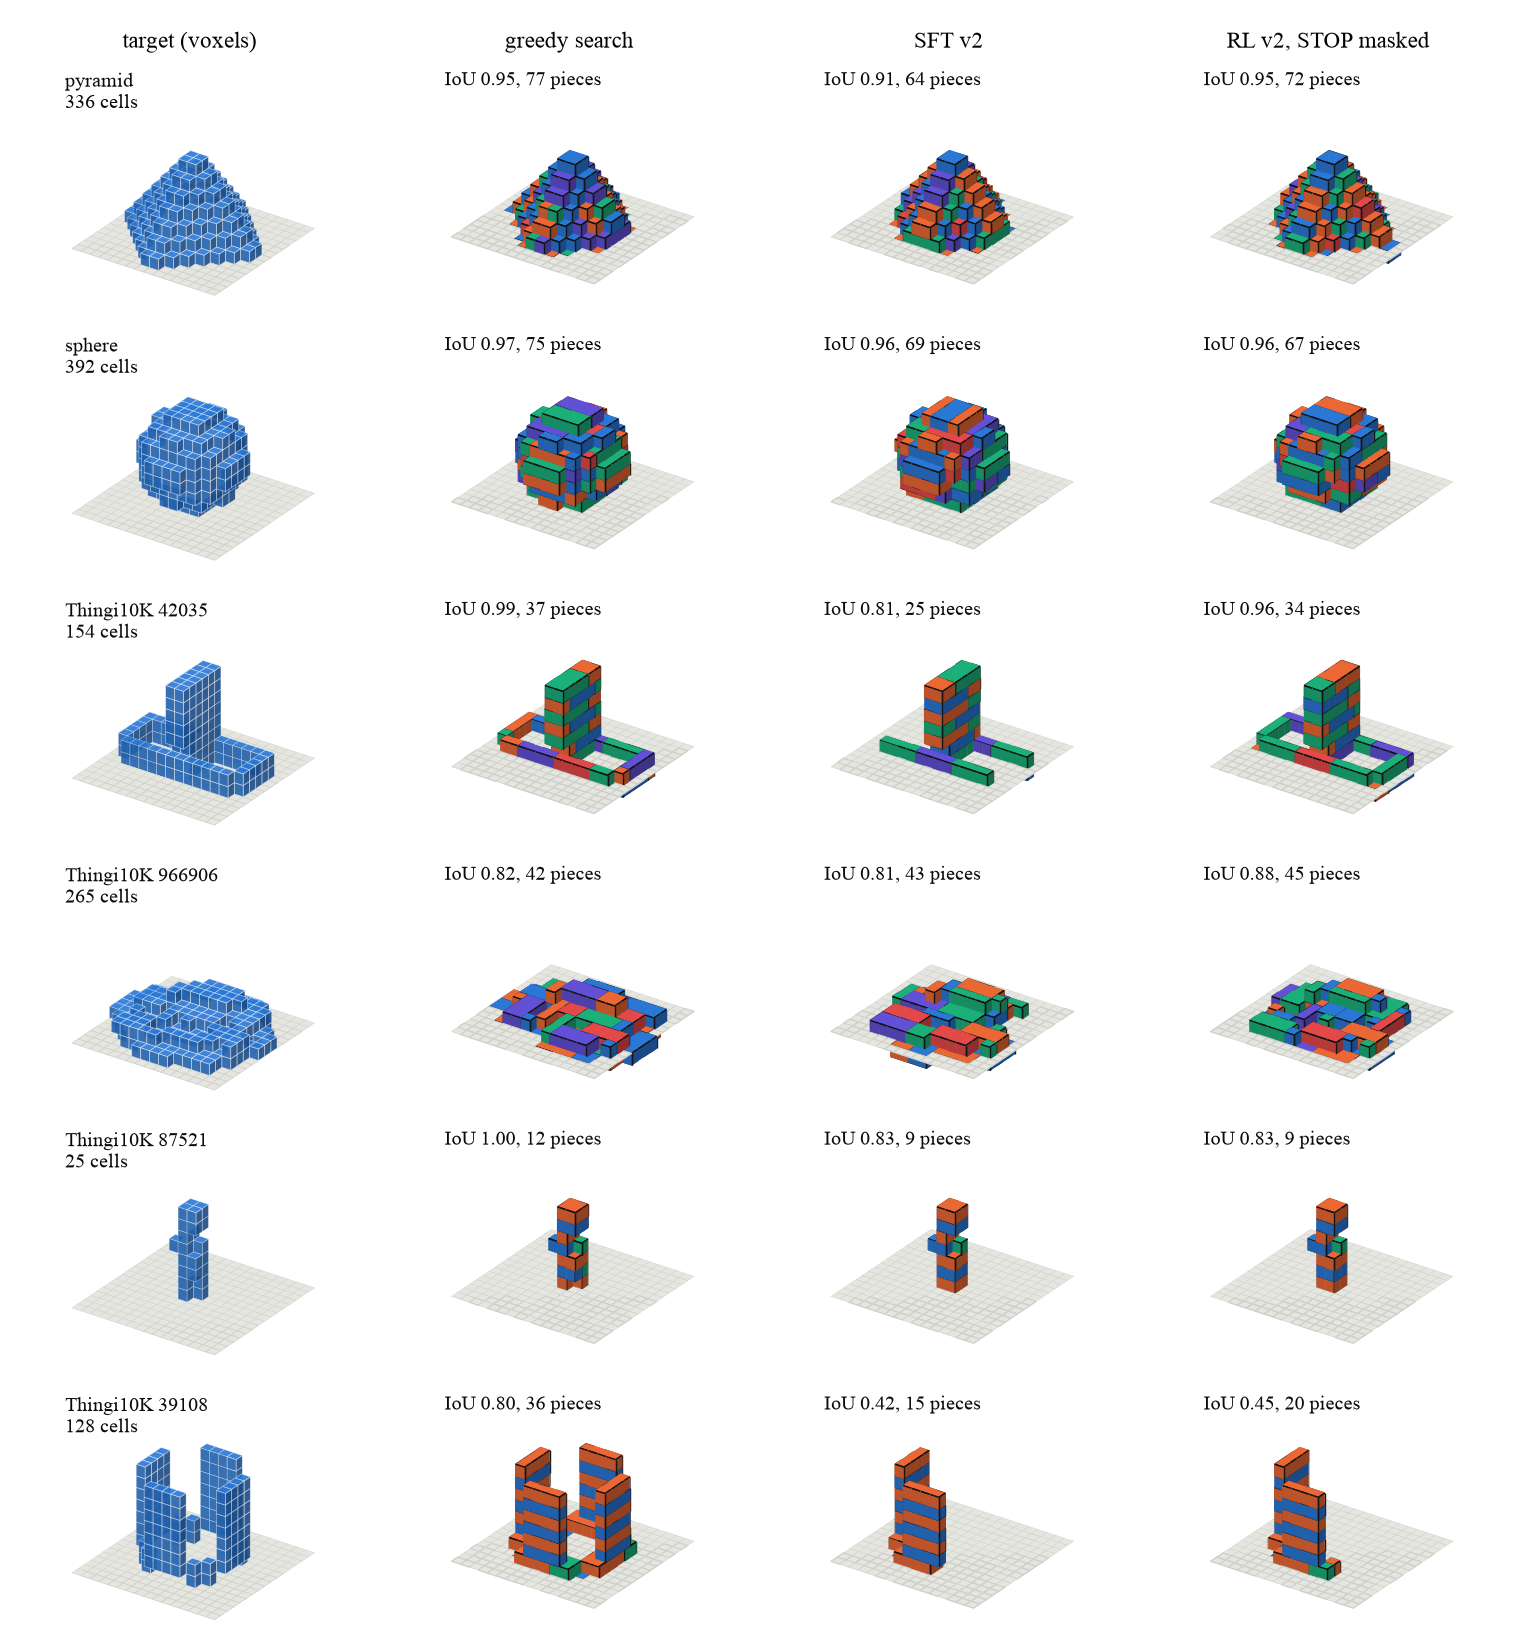
\includegraphics[width=\linewidth]{gallery}
  \caption{Six benchmark cases at the 200-piece cap: the voxel target, the search, SFT v2 and RL v2 with STOP masked.
  Rows: two procedural shapes (the pyramid shows SFT dropping pieces that RL recovers), a mesh where RL recovers most
  of SFT's loss (T42035), the largest RL win (T966906), a small mesh lost by both learned arms (T87521), and the
  honeycomb pot (T39108), the one case any learned generator loses by more than 0.35. Colours separate neighbouring
  bricks and carry no meaning.}
  \label{fig:gallery}
\end{figure}

Figure~\ref{fig:gallery} shows where the remaining gap lives. Twelve cases are lost to the search in both seeds: two
procedural shapes by at most 0.02 (sphere, wedge) and ten real meshes. One shape class dominates: thin-walled shells
with interior structure. The honeycomb pot (T39108) is the only case any learned generator loses by more than 0.35
(search 0.80, RL 0.45 and 0.42 across seeds): the policy tiles the outer walls as it would a solid and 19 of its 39
pieces are removed by the trim as unconnected. The search's exhaustive scan of every placement at every step, with
hard cells first, still beats a learned preference on such shapes. The six real meshes won in both seeds are the
opposite: broad, low shapes where the policy's placements interlock better than the search's layer-wise tiling and
the trim removes less. Finally, the two cases that are valid but unstable under the model for every generator are
tiny fragments (3 to 5 pieces with overhangs) left after trimming a mesh that occupies fewer than 90 of the 2048
cells; grid resolution, not the generator, is the limit there.

\section{Negative results and limitations}
\label{sec:limitations}

We state these as findings rather than caveats, because each one changes what the headline means.

\begin{itemize}
  \item \textbf{Learned stopping is unsolved.} After imitation, after RL on a half-real-mesh episode mix, and in
  both ablations, the policy's own stop action ends some real-mesh builds at zero pieces. The reported numbers use a
  masked stop and thereby borrow the search's stopping rule. A policy that knows when it is done remains future work.
  \item \textbf{The stability bonus did nothing.} Stability under the model is produced by the legality rules and the
  trim; the reward term is redundant here. We did not test harder settings (plates, overhanging parts, larger
  grids) where it might matter.
  \item \textbf{The connectivity features' benefit is only visible off the benchmark mean.} Their effect is clear in the
  policy's own stopping, on the larger held-out split and head to head, but a reader who looks only at
  Table~\ref{tab:ablations}'s mean would conclude they are useless. Fifty-two cases are too few to resolve a 0.02
  effect when one case can move by 0.3.
  \item \textbf{Stability is a model, not a test.} The force model uses a literature clutch constant, ignores lateral
  loads, friction and deformation, and no build was assembled physically. Every ``stable'' in this paper means
  \stablenote.
  \item \textbf{The learned policies are distilled from the search.} ``Learned versus hand-engineered'' is really
  learned-from-hand-engineered: the imitation targets are the search's builds, and RL starts from that policy with a
  KL penalty towards it. The policy did not discover a different style of building; it got better at the search's.
  \item \textbf{Small benchmark, few seeds.} Fifty-two attempted cases, two training seeds for the v2 ladder, one
  seed for the v1 arms and the ablations, one decode seed (decoding is deterministic). Differences below about 0.02
  should be read as observed, not established. We report ranges, not confidence intervals.
  \item \textbf{A small world.} One grid (16\,$\times$\,16\,$\times$\,8), solid fill, six upright bricks, one colour, no
  plates or slopes, no inventory constraints. Thin objects occupy 20 to 90 of 2048 cells and fragment at this
  resolution; grid resolution is the main lever and was not varied.
  \item \textbf{Three budget points, and the largest rarely binds.} The budget study has three points, and at 200 the
  cap is almost never the stopping reason. A finer sweep below 100 pieces would say more about the trade-off.
  \item \textbf{Comparable, not equal, decode cost.} The policy takes about twice the search's time per shape, both
  under 0.2\,s. Best-of-8 sampling from the SFT policy nearly matches RL at about seven times the cost, so RL's
  advantage is cost, not a higher ceiling.
  \item \textbf{Thingi10K has no semantic categories.} The 40 meshes are a deterministic draw from the licensed,
  watertight subset, not a curated set of recognisable objects, and one benchmark is not a general claim.
\end{itemize}

\section{Related work}
\label{sec:related}

% Placeholder until the literature search report is in; see paper/related_work_report.md.
Brick-model generation from 3D shapes has been studied as an optimisation problem and, more recently, as a learning
problem; stability of brick assemblies has its own line of work, from which our force model is taken
\citep{liu2024stablelego}; and the training recipe we use, imitation followed by PPO fine-tuning with a KL penalty
towards the initial policy, follows a pattern established elsewhere \citep{schulman2017ppo}. A full survey of these
three lines, with the works this paper builds on, is given here once the literature pass is complete.

\section{Conclusion}

Inside one fixed pipeline of legality rules, a connected-component trim, an assembly planner, a validator and a
simplified stability model, a 100k-parameter candidate-scoring policy trained for under five hours on a laptop builds
brick models within 0.012 mean IoU of a hand-engineered search at comparable decode cost, with identical validity and
model-stability counts, reproduced across two training seeds. Fidelity saturates between 100 and 200 pieces for
every generator because the cap rarely binds. Reinforcement learning on the fidelity of the finished build supplied
most of the gain beyond imitation, and rebalancing the data towards real meshes supplied the rest; the stability
reward supplied nothing, because the hard constraints already enforce it. The policy's own stop action remains the
open problem, and thin-walled shells remain the search's. The benchmark, its audit, the training recipes and the
figure scripts are released so that every number here can be regenerated.


\bibliographystyle{plainnat}
\bibliography{refs}

\appendix
\section{Benchmark suite}
\label{app:suite}
\paragraph{Procedural fixtures (13).} cube (8\,$\times$\,8\,$\times$\,4 grid), slab, tower, L shape, T shape, wedge
(simple solids, expected valid with coverage at least 0.8); pyramid, sphere (overhangs); cylinder (budget-limited,
coverage at least 0.5); bridge; flat sheet (cannot be covered, expected partial); thin pole (zero valid builds,
expected no valid candidate); open box (non-watertight, expected rejected at parse time). The last is the one case
excluded from every mean; the thin pole is attempted and scores 0 for every generator.

\paragraph{Thingi10K subset (40).} Drawn with seed 0 from the Hugging Face mirror of Thingi10K among models that are
CC BY, CC BY-SA or public domain, closed, manifold, single-component solids with 100 to 200k faces, one file per
Thingiverse object, all with $+z$ up. Licence, author, name and source link are stored per model in the benchmark
records. The meshes are downloaded by a script and never redistributed.

\section{Hyperparameters and cost}
\label{app:hparams}
\begin{table}[h]
  \centering\small
  \begin{tabular}{@{}p{0.14\linewidth}p{0.84\linewidth}@{}}
    \toprule
    \textbf{Policy} & 4\,$\times$ Conv3d($3^3$, 32 ch) + GELU; candidate MLP 64-64-1 on pooled features + 13 (15 in RL)
    candidate features; STOP and value MLPs 64-1 on global mean + max; 97{,}058 parameters (101{,}283 with the RL
    layout and value head) \\
    \textbf{SFT} & teacher forcing, cross-entropy over candidates + STOP; AdamW $10^{-3}$, cosine schedule, batch 32,
    20{,}000 steps, grad clip; 8-fold symmetry augmentation; streaming item pool; free-run eval every 1000 steps on 64
    examples; v2 draws half of each pool refresh from real meshes and drops examples whose teacher covers under half
    the target \\
    \textbf{RL} & PPO, clip 0.2, entropy 0.01, KL 0.05 to the frozen initial policy, value coefficient 0.5, Adam
    $10^{-4}$, grad clip 1.0, $\gamma = 1$ (terminal reward), advantages normalised per batch; 250 iterations
    $\times$ 128 episodes, temperature 1, 8 forked CPU rollout workers, 3 epochs, minibatch 128; reward IoU after trim
    + 0.1 $\cdot$ stable; eval every 10 iterations on 64 examples (half real in v2); best checkpoint by eval IoU \\
    \textbf{Data} & v1: 2000 procedural + 150 real (at most 50k faces, teacher coverage at least 0.5), split
    1750 / 194 / 206. v2: 2000 procedural + 640 real (at most 200k faces, weak-teacher targets kept with their
    coverage recorded), split 2132 / 248 / 260 (test: 188 procedural, 72 real of which 30 weak-teacher) \\
    \textbf{Hardware} & one Apple M5 Pro laptop, 24\,GB; SFT and PPO updates on Metal, rollouts and all benchmark
    decoding on CPU for bit-reproducibility \\
    \textbf{Wall clock} & SFT 23 to 28 min per run; RL v1 2\,h\,25\,min, RL v2 1\,h\,35\,min (seed 0) and
    2\,h\,22\,min (seed 1), ablations about 2\,h\,25\,min each; the frozen benchmark 60\,s for the search and a few
    minutes per learned generator; the audit regenerates every record in a comparable time \\
    \bottomrule
  \end{tabular}
\end{table}

\section{The decode decision}
\label{app:stop}
\begin{table}[h]
  \centering\small
  \caption{The decode decision. Mean IoU after trim on the SFT test split (260 examples at the 100-piece cap: 188
  procedural, 72 real meshes, of which 30 have a teacher build covering under half the target), for the learned stop
  and for masked stop. Made before any benchmark run of the checkpoint.}
  \label{tab:stop}
  \footnotesize
  \begin{tabular}{llcccc}
    \toprule
    checkpoint & STOP & all & procedural & real & real, weak teacher \\
    \midrule
    greedy teacher & -- & 0.843 & 0.943 & 0.584 & -- \\
    SFT v1 & learned / masked & 0.770 / 0.775 & 0.863 / 0.864 & 0.527 / 0.543 & 0.175 / 0.184 \\
    SFT v2 & learned / masked & 0.766 / 0.782 & 0.870 / 0.876 & 0.493 / 0.535 & 0.123 / 0.179 \\
    RL v1 & learned / masked & 0.824 / 0.835 & 0.936 / 0.936 & 0.531 / 0.569 & 0.190 / 0.206 \\
    RL v2, seed 0 & learned / masked & 0.828 / 0.840 & 0.937 / 0.939 & 0.542 / 0.581 & 0.147 / 0.208 \\
    RL v2, seed 1 & learned / masked & 0.821 / 0.835 & 0.931 / 0.935 & 0.533 / 0.574 & 0.141 / 0.204 \\
    RL v2, no stability reward & learned / masked & 0.834 / 0.842 & 0.940 / 0.941 & 0.559 / 0.587 & 0.188 / 0.223 \\
    RL v2, no connectivity inputs & learned / masked & 0.766 / 0.805 & 0.885 / 0.906 & 0.455 / 0.543 & 0.129 / 0.197 \\
    \bottomrule
  \end{tabular}
\end{table}

\section{Stability model}
\label{app:stability}
Bricks are rigid and loaded by their own weight (2.32\,g per 2\,$\times$\,4 brick, scaled by footprint area).
Each shared stud cell between an upper and a lower brick carries vertical force at four sub-points near the cell
corners; ground cells carry compression only. Per brick, vertical force balance and torque balance about $x$ and $y$
are imposed. A linear program finds the smallest tension utilisation $t$ such that every joint force lies in
$[-t\,T/4,\,+\infty)$ with $T = 0.98$\,N per stud cell. StableLego~\citep{liu2024stablelego} measured 0.98\,N as the
capacity of one contact point (three to four per stud), so dividing it over four points per stud makes this model
about four times more conservative than theirs; we keep the conservative reading because no capacity was measured in
this project.
$t \le 1$ is reported as stable under the model; an infeasible program even with unlimited tension means the centre
of mass has left the support (topple). The model has no lateral loads, shear, friction, deformation, hand forces or
dynamics, and its constants were not measured on any physical brick in this project. One program takes about 20\,ms
for a 75-piece build.

\section{Assembly planner}
\label{app:planner}
Rules: one brick per step, inserted straight down onto a horizontal work surface, starting from a ground brick. A
brick may be added when it does not collide, attaches to the assembled component (ground contact or studs of a placed
brick directly below), its vertical insertion path is clear, and it does not seal an unplaced brick beneath it. The
last rule is an exact dead-end test, which makes greedy selection complete: if any full order exists, the first
unplaced brick of that order is always attachable and safe, so the planner never backtracks. Ties break on lowest
layer, then most placed supporters, then id, which gives a layer-by-layer order. For this catalogue (same-height
upright bricks, every non-ground brick supported from below) every structurally valid build has a planned order; the
validator replays the steps and checks the insertion path.

\section{Reproducibility}
\label{app:repro}
All code, benchmark records, audit logs and figure scripts are in the repository. The commands below regenerate the
paper's numbers from a fresh checkout (training needs the Thingi10K download, about 1.5\,GB, and the laptop GPU):
\begin{verbatim}
make bench                                   # frozen greedy baseline + audit
make sft-train sft-bench rl-train rl-bench   # v1 ladder
make data-v2 sft-train-v2 rl-train-v2 \
     rl-bench-v2                             # v2 ladder, seed 0
make v2-seed1 rl-bench-v2-seeds              # v2 ladder, seed 1
make rl-ablations rl-bench-v2-ablations      # ablations
make paper-builds paper-figs paper-check \
     paper-pdf                               # figures, macros, checks, this PDF
\end{verbatim}
Every number in the main tables is a macro written by the figure script from the benchmark records, so the text
cannot drift from the data. Decoding runs on CPU and is bit-identical across processes; voxelization pins the random
state used by the containment test. The benchmark files are the six \code{.jsonl} files under \code{docs/benchmarks/} named in Section~\ref{sec:benchmark}.

\section{Per-case results}
\label{app:percase}
% generated by paper/scripts/figs.py tables; do not edit
Per-case IoU after trim at the 200-piece cap (0 for a missing or invalid build). RL columns use the masked stop; cells is the number of occupied target cells out of 2048 (512 for the cube).
\begin{center}\footnotesize\setlength{\tabcolsep}{4pt}
\begin{tabular}{llrcccccc}
\toprule
case & source & cells & search & SFT v2 & RL v2 s0 & RL v2 s1 & no stab. & no conn. \\
\midrule
bridge & procedural & 224 & 0.964 & 0.964 & 0.964 & 0.964 & 0.964 & 0.964 \\
cube & procedural & 256 & 1.000 & 0.641 & 1.000 & 1.000 & 1.000 & 1.000 \\
cylinder & procedural & 608 & 1.000 & 1.000 & 1.000 & 1.000 & 1.000 & 1.000 \\
flat\_sheet\_impossible & procedural & 160 & 0.050 & 0.050 & 0.050 & 0.050 & 0.050 & 0.050 \\
l\_shape & procedural & 540 & 1.000 & 1.000 & 1.000 & 1.000 & 1.000 & 1.000 \\
pyramid & procedural & 336 & 0.946 & 0.911 & 0.946 & 0.928 & 0.918 & 0.911 \\
slab & procedural & 480 & 1.000 & 1.000 & 1.000 & 1.000 & 1.000 & 1.000 \\
sphere & procedural & 392 & 0.975 & 0.959 & 0.957 & 0.954 & 0.959 & 0.964 \\
t\_shape & procedural & 288 & 1.000 & 1.000 & 1.000 & 1.000 & 1.000 & 1.000 \\
thin\_pole & procedural & 0 & 0.000 & 0.000 & 0.000 & 0.000 & 0.000 & 0.000 \\
tower & procedural & 32 & 1.000 & 1.000 & 1.000 & 1.000 & 1.000 & 1.000 \\
wedge & procedural & 192 & 1.000 & 0.990 & 0.995 & 0.995 & 0.990 & 0.995 \\
T100070 & thingi10k & 1070 & 1.000 & 0.938 & 1.000 & 1.000 & 0.999 & 0.998 \\
T100894 & thingi10k & 84 & 0.913 & 0.905 & 0.907 & 0.905 & 0.907 & 0.907 \\
T105120 & thingi10k & 56 & 0.200 & 0.267 & 0.194 & 0.271 & 0.194 & 0.138 \\
T108578 & thingi10k & 68 & 0.057 & 0.000 & 0.057 & 0.057 & 0.057 & 0.057 \\
T108884 & thingi10k & 276 & 0.953 & 0.931 & 0.933 & 0.953 & 0.971 & 0.932 \\
T110201 & thingi10k & 32 & 0.250 & 0.250 & 0.250 & 0.273 & 0.250 & 0.250 \\
T111878 & thingi10k & 60 & 0.109 & 0.109 & 0.109 & 0.109 & 0.109 & 0.108 \\
T1130077 & thingi10k & 205 & 0.698 & 0.718 & 0.718 & 0.718 & 0.718 & 0.718 \\
T113134 & thingi10k & 108 & 0.404 & 0.393 & 0.460 & 0.327 & 0.414 & 0.447 \\
T130960 & thingi10k & 184 & 0.967 & 0.968 & 0.968 & 0.947 & 0.957 & 0.968 \\
T1335002 & thingi10k & 400 & 0.980 & 0.946 & 0.950 & 0.947 & 0.941 & 0.948 \\
T1417953 & thingi10k & 256 & 1.000 & 1.000 & 1.000 & 1.000 & 1.000 & 1.000 \\
T144106 & thingi10k & 64 & 0.300 & 0.210 & 0.308 & 0.316 & 0.316 & 0.333 \\
T1514900 & thingi10k & 92 & 0.706 & 0.593 & 0.652 & 0.702 & 0.652 & 0.626 \\
T200212 & thingi10k & 365 & 0.989 & 0.981 & 0.992 & 0.986 & 0.984 & 0.981 \\
T225935 & thingi10k & 290 & 0.907 & 0.852 & 0.883 & 0.865 & 0.888 & 0.837 \\
T265728 & thingi10k & 49 & 0.648 & 0.571 & 0.588 & 0.588 & 0.588 & 0.635 \\
T39108 & thingi10k & 128 & 0.800 & 0.420 & 0.448 & 0.420 & 0.250 & 0.780 \\
T39922 & thingi10k & 168 & 0.667 & 0.964 & 0.667 & 0.667 & 0.661 & 0.667 \\
T40447 & thingi10k & 452 & 1.000 & 1.000 & 1.000 & 1.000 & 1.000 & 1.000 \\
T42025 & thingi10k & 84 & 0.024 & 0.023 & 0.023 & 0.035 & 0.023 & 0.023 \\
T42035 & thingi10k & 154 & 0.987 & 0.808 & 0.957 & 0.727 & 0.807 & 0.662 \\
T48124 & thingi10k & 37 & 0.295 & 0.295 & 0.311 & 0.295 & 0.311 & 0.311 \\
T53749 & thingi10k & 278 & 0.458 & 0.439 & 0.449 & 0.432 & 0.387 & 0.449 \\
T54820 & thingi10k & 82 & 0.427 & 0.427 & 0.427 & 0.546 & 0.427 & 0.427 \\
T56630 & thingi10k & 359 & 0.955 & 0.978 & 0.978 & 0.975 & 0.978 & 0.943 \\
T567026 & thingi10k & 20 & 0.200 & 0.000 & 0.200 & 0.200 & 0.200 & 0.200 \\
T61192 & thingi10k & 26 & 1.000 & 1.000 & 1.000 & 1.000 & 1.000 & 1.000 \\
T69537 & thingi10k & 64 & 0.812 & 0.778 & 0.788 & 0.866 & 0.778 & 0.778 \\
T70559 & thingi10k & 13 & 0.231 & 0.231 & 0.231 & 0.231 & 0.231 & 0.200 \\
T71307 & thingi10k & 76 & 0.237 & 0.224 & 0.272 & 0.350 & 0.350 & 0.330 \\
T75090 & thingi10k & 238 & 0.790 & 0.701 & 0.793 & 0.810 & 0.778 & 0.800 \\
T75651 & thingi10k & 125 & 0.920 & 0.921 & 0.931 & 0.936 & 0.929 & 0.929 \\
T80597 & thingi10k & 188 & 0.883 & 0.819 & 0.851 & 0.856 & 0.841 & 0.815 \\
T81589 & thingi10k & 212 & 0.972 & 0.972 & 0.972 & 0.967 & 0.963 & 0.968 \\
T87521 & thingi10k & 25 & 1.000 & 0.833 & 0.833 & 1.000 & 0.926 & 0.926 \\
T91350 & thingi10k & 433 & 0.993 & 0.984 & 0.986 & 0.989 & 0.973 & 0.984 \\
T91452 & thingi10k & 42 & 0.159 & 0.159 & 0.159 & 0.109 & 0.159 & 0.159 \\
T93881 & thingi10k & 91 & 1.000 & 1.000 & 1.000 & 1.000 & 1.000 & 1.000 \\
T966906 & thingi10k & 265 & 0.817 & 0.814 & 0.879 & 0.773 & 0.896 & 0.782 \\
\midrule
mean & & & 0.705 & 0.672 & 0.693 & 0.693 & 0.686 & 0.690 \\
\bottomrule
\end{tabular}
\end{center}



\end{document}
